\section{Main Results and Predictions}

Our theoretical model yields two central results with direct empirical implications for the persistence and variation of algorithmic bias. The analysis hinges on the firm's optimization problem, where we formally establish that the profit-maximizing value function, $V(b)$, is strictly concave (see Lemma 3 in the Appendix). This ensures a unique, interior solution for the optimal level of bias, which we characterize below.

\begin{proposition}[Existence of Optimal Bias]
\label{prop:existence}
For any fairness-accuracy trade-off ($\kappa > 0$), a profit-maximizing firm's optimal choice of bias is strictly positive ($b^* > 0$).
\end{proposition}
\begin{proof}
See Appendix A.3. The proof shows that at zero bias, the marginal value of increasing bias is strictly positive ($dV/db|_{b=0} > 0$). Given the concavity of $V(b)$, the optimum must be an interior solution.
\end{proof}

This proposition provides our first key prediction: \textbf{Firms will rationally choose to employ biased algorithms even when groups have identical average productivity and debiasing is costless.} This outcome is not driven by animus or priors, but by the informational value gained from the precision-bias trade-off inherent in the technology.

\begin{proposition}[Comparative Static on the Trade-off]
\label{prop:comparative_static}
The optimal level of bias $b^*$ is increasing in the severity of the fairness-accuracy trade-off, $\kappa$.
\end{proposition}
\begin{proof}
See Appendix A.4. The proof uses the Implicit Function Theorem on the first-order condition to show that $\partial b^*/\partial\kappa > 0$.
\end{proof}

This result generates a set of powerful, testable predictions about where and why bias should vary. 
First, \textbf{firms or industries operating in environments with a steeper trade-off (a higher $\kappa$) will choose higher levels of bias, all else equal.} This might occur in contexts where prediction is inherently more complex or data is less balanced.
Second, and conversely, \textbf{technological improvements that flatten the fairness-accuracy trade-off (i.e., lower $\kappa$) should lead to measurable reductions in observed bias levels,} as the marginal benefit of retaining bias diminishes.

These predictions distinguish our informational mechanism from alternative explanations based on taste-based or statistical discrimination. The key empirical hurdle would be to validate the existence and measure the steepness ($\kappa$) of the precision-bias trade-off across different domains and implementations.

The model's mechanics and the intuition behind these results are summarized in Figure \ref{fig:main_results}.

\begin{figure}[H]
\centering
\begin{subfigure}{0.48\textwidth}
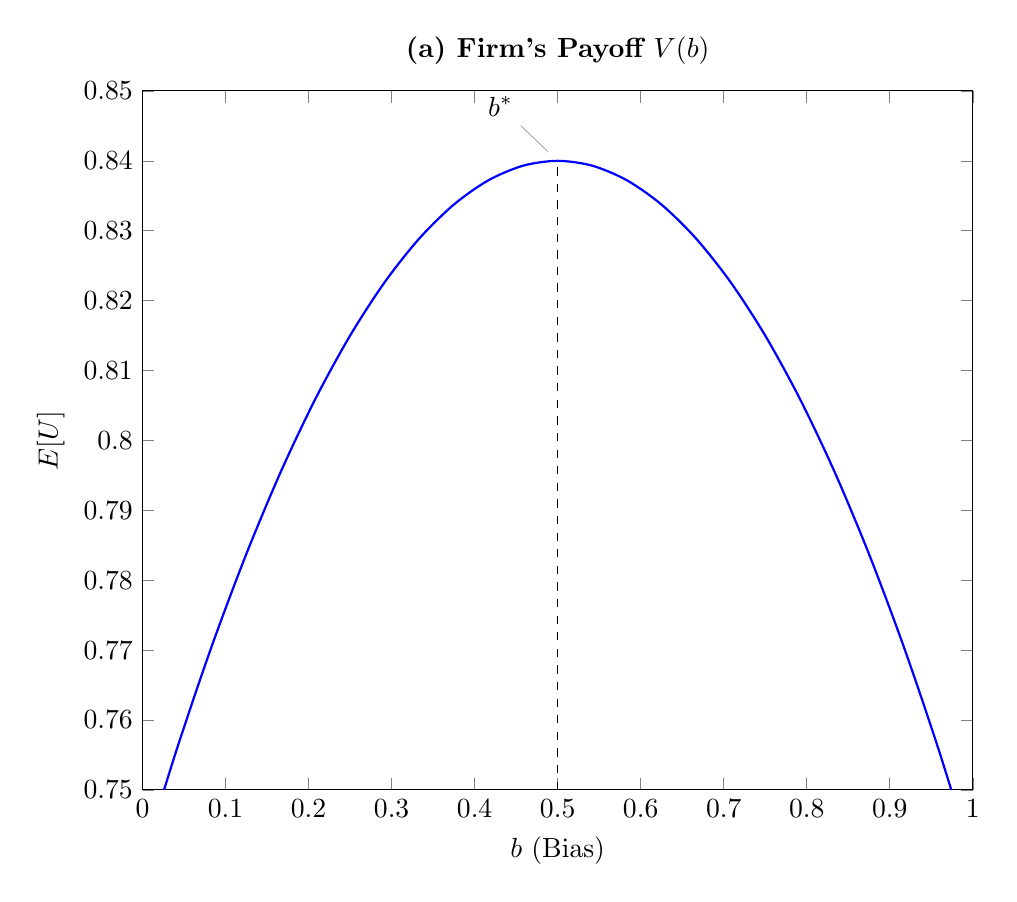
\begin{tikzpicture}
\begin{axis}[title={\textbf{(a) Firm's Payoff $V(b)$}}, xlabel={$b$ (Bias)}, ylabel={$\mathbb{E}[U]$}, xmin=0, xmax=1, ymin=0.75, ymax=0.85, legend pos=south east, width=\linewidth]
    \addplot[smooth, thick, color=blue, domain=0:1] {-0.4*(x-0.5)^2 + 0.84};
    \node[pin=135:{$b^*$}] at (axis cs:0.5, 0.84) {};
    \draw[dashed] (axis cs:0.5,0.75) -- (axis cs:0.5,0.84);
\end{axis}
\end{tikzpicture}
\end{subfigure}% <-- No blank line here
\hfill
\begin{subfigure}{0.48\textwidth}
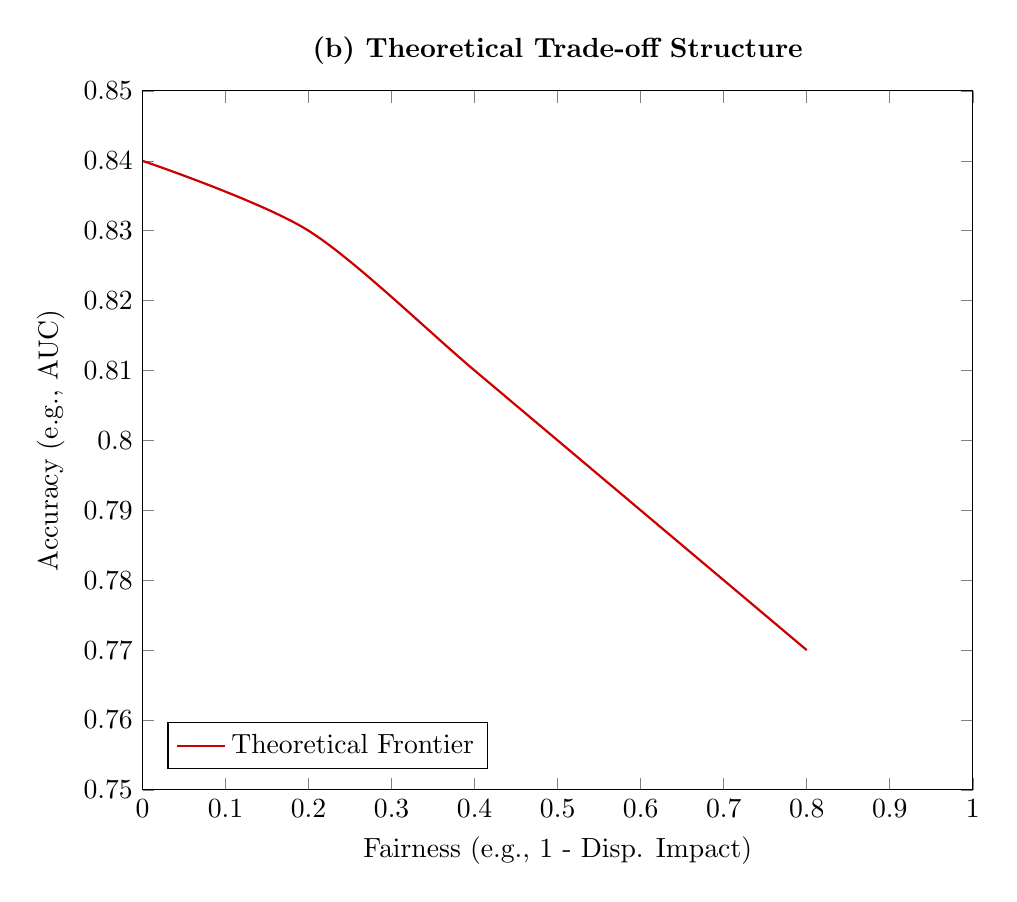
\begin{tikzpicture}
\begin{axis}[title={\textbf{(b) Theoretical Trade-off Structure}}, xlabel={Fairness (e.g., 1 - Disp. Impact)}, ylabel={Accuracy (e.g., AUC)}, xmin=0, xmax=1, ymin=0.75, ymax=0.85, legend pos=south west, width=\linewidth]
    \addplot[smooth, thick, color=red!80!black] coordinates {(0, 0.84) (0.2, 0.83) (0.4, 0.81) (0.6, 0.79) (0.8, 0.77)};
    \addlegendentry{Theoretical Frontier};
\end{axis}
\end{tikzpicture}
\end{subfigure}

\vspace{1cm}

\begin{subfigure}{0.48\textwidth}
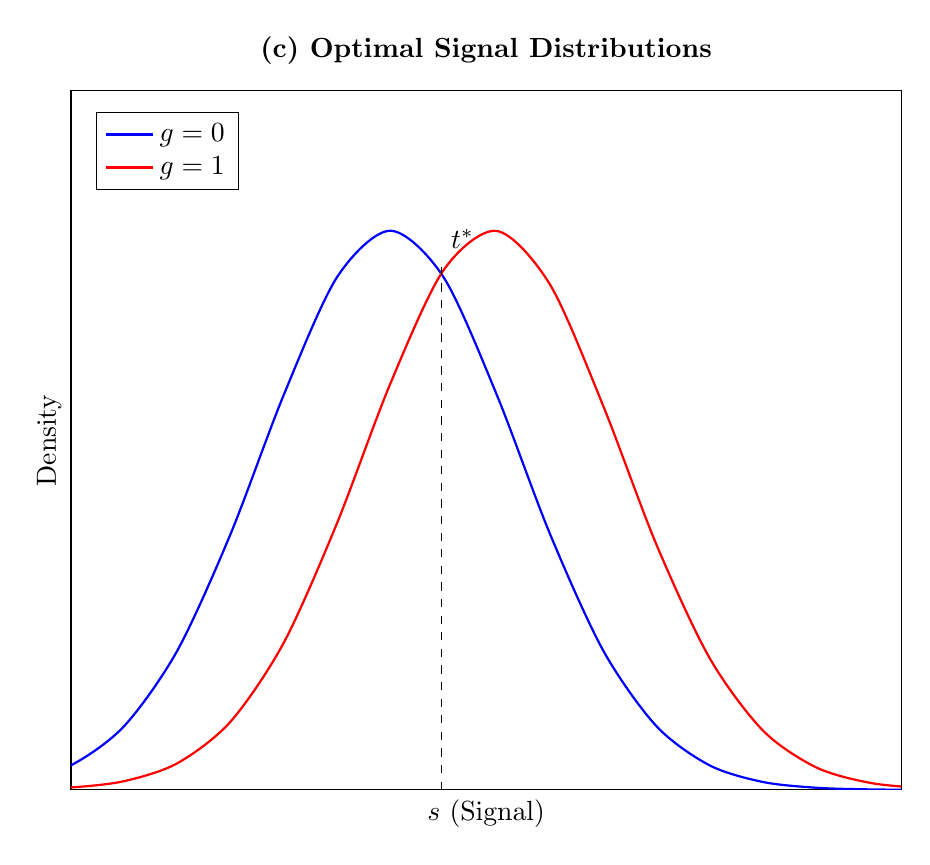
\begin{tikzpicture}
\begin{axis}[title={\textbf{(c) Optimal Signal Distributions}}, xlabel={$s$ (Signal)}, ylabel={Density}, xmin=-2.5, xmax=4, ymin=0, ymax=0.5, xtick=\empty, ytick=\empty, legend pos=north west, width=\linewidth]
    \addplot[smooth, thick, color=blue] {0.4*exp(-(x-0)^2 / (2*1^2))}; \addlegendentry{$g=0$};
    \addplot[smooth, thick, color=red] {0.4*exp(-(x-0.8)^2 / (2*1^2))}; \addlegendentry{$g=1$};
    \draw[dashed] (axis cs:0.4,0) -- (axis cs:0.4,0.38); \node[above right] at (axis cs:0.4,0.38) {$t^*$};
\end{axis}
\end{tikzpicture}
\end{subfigure}% <-- No blank line here
\hfill
\begin{subfigure}{0.48\textwidth}
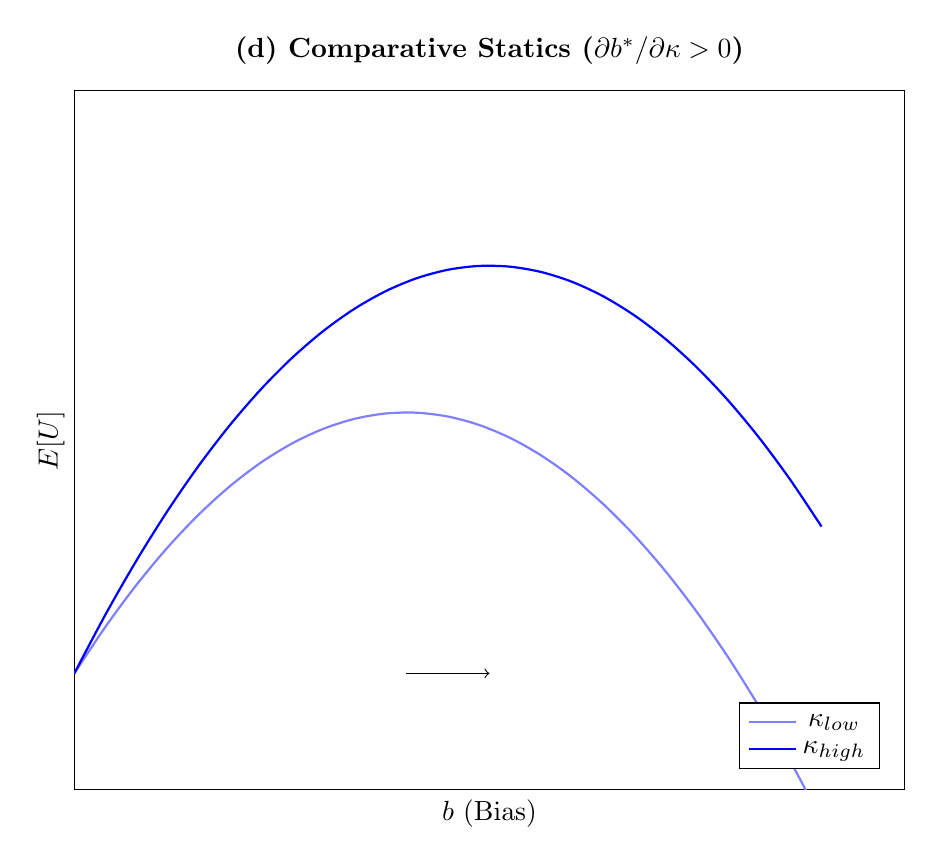
\begin{tikzpicture}
\begin{axis}[title={\textbf{(d) Comparative Statics ($\partial b^*/\partial\kappa > 0$)}}, xlabel={$b$ (Bias)}, ylabel={$\mathbb{E}[U]$}, xmin=0, xmax=1, ymin=0, ymax=0.3, xtick=\empty, ytick=\empty, legend pos=south east, width=\linewidth]
    \addplot[smooth, thick, domain=0:0.9, color=blue!50] {-0.7*x^2 + 0.56*x + 0.05}; \addlegendentry{$\kappa_{low}$}
    \addplot[smooth, thick, domain=0:0.9, color=blue!100] {-0.7*x^2 + 0.7*x + 0.05}; \addlegendentry{$\kappa_{high}$}
    \draw[->, thin] (axis cs:0.4, 0.05) -- (axis cs:0.5, 0.05);
\end{axis}
\end{tikzpicture}
\end{subfigure}
\caption[Model Mechanics and Results]{\textbf{Model Mechanics and Results.} Panel (a): Firm's concave value function $V(b)$ is maximized at $b^* > 0$. Panel (b): The theoretical trade-off structure predicted by the model. Panel (c): Optimal signal distributions for group 0 (blue) and group 1 (red), shifted by $b^*$. Panel (d): A higher $\kappa$ (steeper trade-off) increases optimal bias.}
\label{fig:main_results}
\begin{remark}
Note: The figures presented in this paper are generated by the accompanying `results.py` script. Following the updates to the model to incorporate group-specific measurement error, this script will need to be re-run to produce graphs that accurately reflect the new mathematical framework.
\end{remark}
\end{figure}